%!TeX root = main.tex
%!encoding = UTF-8 Unicode

\section{Technology Study}

\subsection{Influence of Chip Active Area}

\subsection{Influence of Robert Bosch SiC MOSFET Generation}

To demonstrate measurement capability, this subsection compares two SiC MOSFETs with active areas of \SI{5}{mm^2} and \SI{10}{mm^2}. 
The objective is to quantify how variations in active area translate into differences in switching behavior and high-frequency EM emissions.
The active area, the portion of the die used for current conduction, significantly affects device performance.
With increasing active area, the current rating, capacitances, transconductance, and reverse-recovery charge typically increase linearly, while voltage rating and threshold voltage remain largely constant.
First, the time-domain switching behavior is analyzed, followed by the frequency-domain emission spectra.


\subsection*{Time-Domain Analysis}

\begin{figure}[htb]
    \centering
    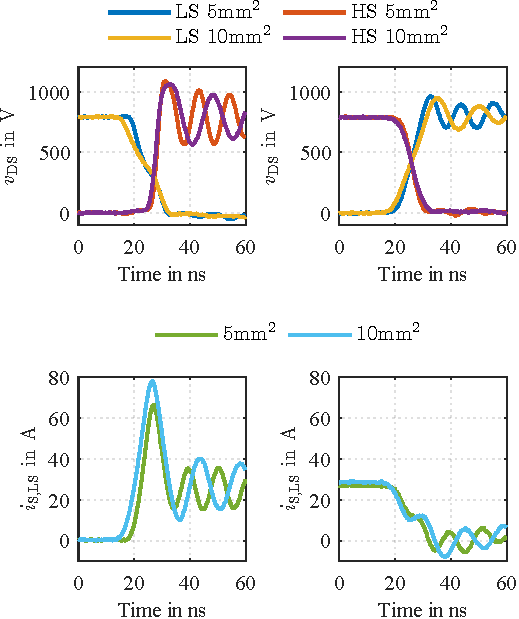
\includegraphics[scale = 1]{figures/7_MeasurementResults/ChipSize_TD_expPDF.pdf}
	\caption{Time-domain low-pass signals for different active areas, measured at \(\mi{V}{DC} = \SI{800}{V}\), \(\mi{I}{L} = \SI{30}{A}\), and \(\mi{T}{amb} = \SI{30}{\celsius}\).}\label{fig:MR_ChipSize_TD}
\end{figure}

Figure~\ref{fig:MR_ChipSize_TD} presents the measured low-pass voltage transients for both devices. 
To enable a fair comparison, both chips are switched with different gate resistances to achieve an equivalent maximum drain-source overvoltage of \SI{1100}{V}, resulting in similar gate time constants:
\begin{equation}
	\mi{\tau}{G} = (\mi{R}{G,int}+\mi{R}{G,ext}) \cdot \mi{C}{iss}
\end{equation}
\begin{align}
	\mi{\tau}{G,\SI{5}{mm^2}} &= \SI{10.8}{\ohm}\,\cdot\,\SI{1.1}{nF} = \SI{11.9}{ns} \\
	\mi{\tau}{G,\SI{10}{mm^2}} &= \SI{6.1}{\ohm}\,\cdot\,\SI{2.2}{nF} = \SI{13.4}{ns}
\end{align}

Despite comparable gate time constants, the larger chip exhibits significantly slower turn-on transients. 
This behavior is dominated by the Miller effect, where the inductive voltage drop causes \mi{v}{DS} to fall substantially, introducing negative feedback to the gate driver. 
The gate driver must charge both the gate-source capacitance and the Miller capacitance:
\begin{equation}
	\frac{\mi{v}{driver}-\mi{v}{GS}}{\mi{R}{G}} \approx \mi{C}{GS} \ddt{\mi{v}{GS}} - \mi{C}{GD} \ddt{\mi{v}{DS}}
\end{equation}
While the first term remains comparable between both devices, the second term is substantially larger for the \SI{10}{mm^2} chip due to its doubled Miller capacitance, explaining the observed slowdown.

Additionally, the passive-off transient of the larger chip exhibits more distorted voltage overshoot, attributed to its higher reverse-recovery charge and resulting inductive drop. 
This elevated reverse-recovery charge is also evident in the larger turn-on current transient.

During active-off switching (right panel of \fref{fig:MR_ChipSize_TD}), a similar trend emerges: the larger chip exhibits slower transients due to its doubled output capacitance. 
Notably, the rise time does not double as expected from classical ZVS theory, since the channel requires finite time to fully turn off. 
The capacitive charging current is thus reduced by the remaining channel current: $\mi{i}{C,DS} = \mi{i}{load} - \mi{i}{channel}$~\cite{van_der_broeck_simulating_2023}.


\subsection*{Frequency-Domain Analysis}

Figure~\ref{fig:MR_ChipSize_FD} shows the high-pass voltage and current spectra with post-processing via the TDF filter. 
Both devices exhibit similar spectral behavior up to \SI{10}{MHz}, where the switching transient begins to dominate. 
At higher frequencies, the effects of different transient speeds can now be quantified: although the \SI{10}{mm^2} device exhibits a higher resonance peak, the \SI{5}{mm^2} device shows significantly higher broadband emissions, reaching up to \SI{14}{dB} at \SI{140}{MHz} for the active low-side switch and \SI{7}{dB} for the passive high-side switch.

\begin{figure*}[htb]
	\centering
	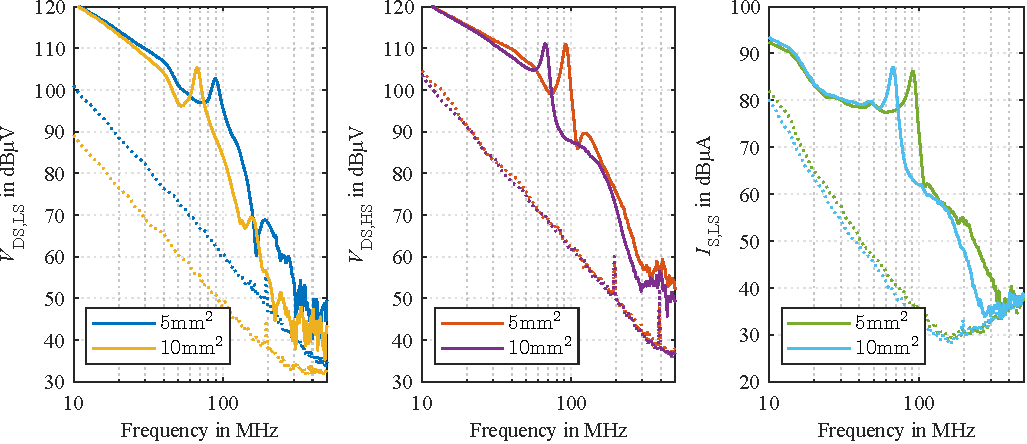
\includegraphics[scale = 1]{figures/7_MeasurementResults/ChipSize_FD_expPDF.pdf}
	% \caption{Frequency domain measurement results of high-pass signals for different active areas.}
	\caption{Frequency-domain high-pass signals for different active areas, measured at \(\mi{V}{DC} = \SI{800}{V}\), \(\mi{I}{L} = \SI{30}{A}\), and \(\mi{T}{amb} = \SI{30}{\celsius}\).}\label{fig:MR_ChipSize_FD}
\end{figure*}

To elucidate this behavior, \fref{fig:MR_ChipSize_SpekZerl_FD} presents the snapped-and-mirrored spectrum of the \SI{5}{mm^2} active LS switch, processed with a peak-detector algorithm~\cite{keller_fast_2007}. 
The spectrum shows that the active-off event dominates at frequencies up to \SI{120}{MHz}, while the active-on event dominates above that. 
Consequently, the reduced impact of the Miller effect and reverse transfer capacitance of the smaller device are the primary drivers of the higher total broadband emission of the smaller chip.

A similar trend is observed in the current spectra, where the \SI{5}{mm^2} device shows \SI{10}{dB} higher broadband emissions up to approximately \SI{270}{MHz}, beyond which measurement noise becomes significant.
At higher frequencies, maintaining sufficient SNR in the current sensor is challenging because higher gain is required to measure the small passive-shunt voltage, compared with the higher output level of the $CR$ divider in the voltage path.
This increased gain of the current sensor comes with increased noise, which limits the highest effectively measurable frequency of the current path compared with the voltage path.

\begin{figure}[ht]
	\centering
	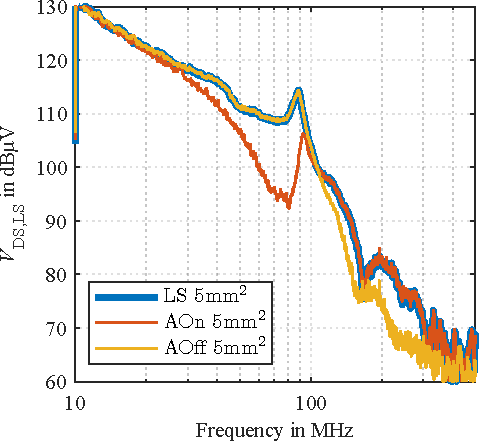
\includegraphics[scale = 1]{figures/7_MeasurementResults/PMTX05_LS_SpekZerl_FD.pdf}
	\caption{Spectrum of the snapped-and-mirrored voltage of the active LS switch with \SI{5}{mm^2} active area. In contrast to the other frequency plots, this spectrum is not a pure Fourier transform; it is post-processed with a peak-detector algorithm~\cite{keller_fast_2007}.}\label{fig:MR_ChipSize_SpekZerl_FD}
\end{figure}



\section{Environmental Study}

\subsection{Influence of Junction-Temperature}

\subsection{Influence of Comutation-Loop Inductance}

\section{Operating-Point Study}


\subsection{Gate Resistance}

\subsubsection{Trade-off: Switching Losses vs. Emissions for Active On}

\subsubsection{Trade-off: Switching Losses vs. Emissions for Active Off}

\subsection{Negative Gate-Driver Bias}

